Dans le but de concrétiser cette approche, on
s'est inspiré d'un modèle\footnote{présenté dans le Ch. 4 du travail réalisé par
\mbox{Guillaume} \mbox{Tisserant} et son équipe}, présenté sur la
figure~\ref{modele_original}, qui représente une vision du fonctionnement que
pourrait avoir une conscience artificielle. En se basant sur des travaux comme
ceux de Freud et de Laborit, il permet de représenter la plupart des caractéristiques
d’une conscience humaine.

Ce modèle peut être vu comme un empilement  de couches de niveau de conscience :
l'inconscient étant la couche la plus basse et le conscient étant la couche la
plus haute. Dans une description plus détaillée de ce modèle, on va préciser la
fonction de chacune de ses couches.

\begin{figure}[H] 
\centering
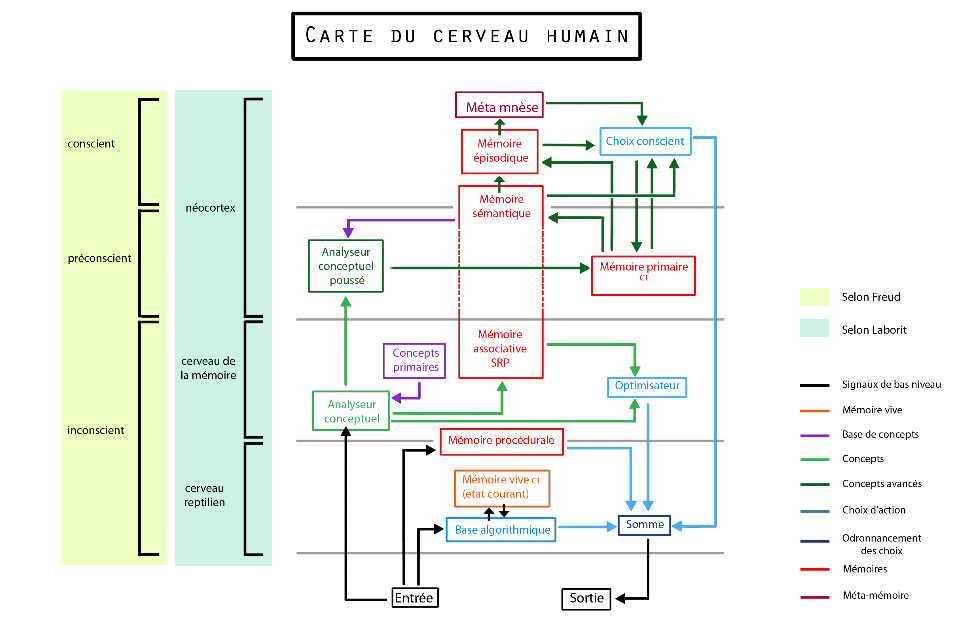
\includegraphics[width=\textwidth]{files/modele_original} 
\caption{Schéma du modèle de représentation de la conscience} 
\label{modele_original}
\end{figure}

\subsection{L’inconscient}
L'inconscient consiste de la couche du cerveau reptilien et celle du cerveau de
la mémoire.
\subsubsection{Le cerveau reptilien} C'est la couche la plus basse du modèle.
\subparagraph{Les entrées/sorties :} Les entrées représentent tout ce qui arrive
au cerveau, que ce soit des percepts externes (les 5 sens), ou interne (pulsions...). Les sorties représentent tout
ce que le cerveau demande de faire au corps. 
\subparagraph{La base algorithmique} est une base
simple qui permet de créer des sorties simples depuis des entrées simples. C’est
ce qui code tous les réflexes innés présents chez un être vivant. La mémoire
procédurale sert à se construire des automatismes en fonction du vécu. Par
exemple, le fait pour un bébé d’apprendre à marcher utilisera la mémoire
procédurale, selon un schéma essai échec.
\subsubsection{Le cerveau de la mémoire} Cette prochaine couche étant plus
complexe que la dernière, ici on trouve un analyseur conceptuel, une mémoire
associative et un optimisateur.
\subparagraph {L'analyseur conceptuel} compare des entrées en dur à une base de
données de concepts primaires (la faim, la soif, le plaisir, la fatigue, la joie, une odeur
nauséabonde, un bruit violent...).
\subparagraph {La mémoire associative} compare la réception de ces concepts
entre eux. Cela permet par exemple à un animal vivant dans un milieu contenant des prédateurs
bruyant d’associer le concept de danger au bruit que fait le prédateur.
\subparagraph {L’optimisateur} a pour vocation d’optimiser un concept qui peut
se traduire par le bien-être. Dans l’exemple précédent, il prend en compte que l’approche d’un
prédateur réduit le bien-être, et que le fait de courir peut éloigner le
prédateur, donc faire remonter le bien être. Il devra donc choisir l’action de
fuir.

\subsection{Le Néocortex : la préconscience et la conscience}
Les couches qui font partie du néocortex représentent la préconscience et la
conscience. C'est ici qu'on s'approche de la cognition humaine.
\subsubsection{Le préconscient} Cette couche consiste d'un analyseur
conceptuel sémantique et des mémoires primaire et sémantique.
\subparagraph{L'analyseur conceptuel sémantique} manipule des concepts un niveau
au dessus de ceux manipulés par l’analyseur conceptuel du cerveau de la mémoire. Il sert à
traduire les concepts primaires en concepts complexes stockés dans la mémoire
sémantique.
\subparagraph{La mémoire sémantique} contient donc une base de
données de concepts avancés, construite sous forme de treillis reliant les concepts ensemble.
\subparagraph{La mémoire primaire} contient un très petit nombre de concepts
sémantiques. Elle contient les choses auxquels auquel une conscience est en
train de penser. Elle peut être remplie par l’analyseur conceptuel sémantique qui lui envoie les
concepts se trouvant dans l’environnement, ou directement par la réflexion
consciente qui choisit d’y poser un concept pour réfléchir dessus.
\subparagraph{La gestion de la mémoire sémantique} est complexe : les concepts
en mémoire primaire sont copiés en mémoire sémantique instantanément. Tout ce qui est en
mémoire primaire y arrive, mais les choses sont aussi oubliées petit à petit.
Plus elles restent ou repassent en mémoire primaire, moins elles disparaissent
de la mémoire sémantique.
\subsubsection{Le conscient} Dans cette couche se trouvent les modules les plus
avancés du modèle : la mémoire épisodique, la méta Mnèse  et le choix conscient.
\subparagraph{La mémoire épisodique} est une mémoire des situations. Elle sert à
se remémorer des situations et des émotions vécus sous formes de concepts sémantiques. Les
concepts stockés viennent à la fois des percepts mais aussi de l’état interne de
la personne au moment de l’événement. Elle gère la persistance de la même
manière que la mémoire sémantique.
\subparagraph{La méta Mnèse} est la mémoire de la mémoire. Son rôle est de stocker la
façon dont les éléments se sont enchaînés dans la mémoire épisodique.
\subparagraph{Le choix conscient} (ou réflexion consciente) ressemble à l'optimisateur,
mais maniant des concepts de plus hauts niveaux, et de natures différentes. Grâce à
la méta Mnèse, il peut utiliser des séries de situations, et même imaginer des
situations passées, présentes ou futures pour prendre des décisions. Il peut
ainsi comparer des situations imaginaires et choisir celle vers laquelle il a
envie de tendre. Il peut aussi réfléchir sur des concepts abstraits, comme sur
ses réflexions passés. Il peut analyser son propre fonctionnement à partir du
moment où il arrive à le retranscrire sous forme de concepts.

\section{Synthèse}
L’objet représenté par \textbf{Somme} dans la couche du cerveau reptilien
est une simplification du schéma retour. Il représente la transformation de tous les
signaux en signaux de bas niveaux, et gère la somme des signaux pour choisir
lesquels inhiber et lesquels renvoyer en sortie. Son fonctionnement nécessite
d’arriver à combiner les signaux entre eux. Par exemple, si une personne choisit
de fumer dans le choix conscient, il doit récupérer la façon d’allumer un
briquet dans la mémoire procédurale.
